\chapter{Results and evaluation}
\label{chap:ResultsAndEvaluation}
\section{Image results}
\label{sec:ImageResults}
%todo add images
Figure \ref{fig:UniversityCampus} shows an overview of the TU/e campus. This is a basic view of the campus. The river dommel is also shown through the campus. This picture is taken above the train tracks.

\begin{figure}[htb!]
\centering
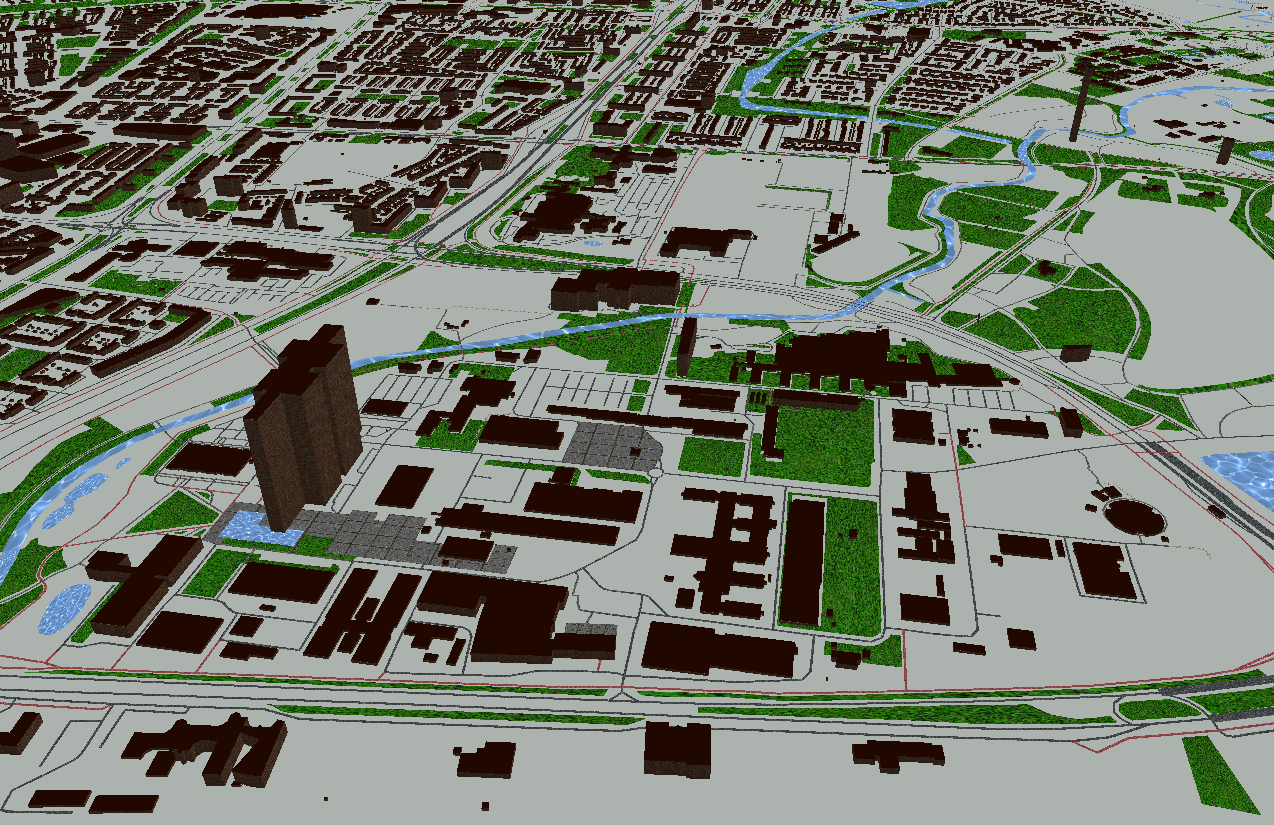
\includegraphics[width=\textwidth]{TUe}
\caption{University campus}
\label{fig:UniversityCampus}
\end{figure} 

The error that is introduced when rendering from a distance is visible in figure \ref{fig:Simplification}. The top image is rendered with less error than the bottom version. In the simplified version, it is possible to see that the building is only a convex hull of its original. Also the roads that are besides the building are removed.

\begin{figure}[htb!]
\centering
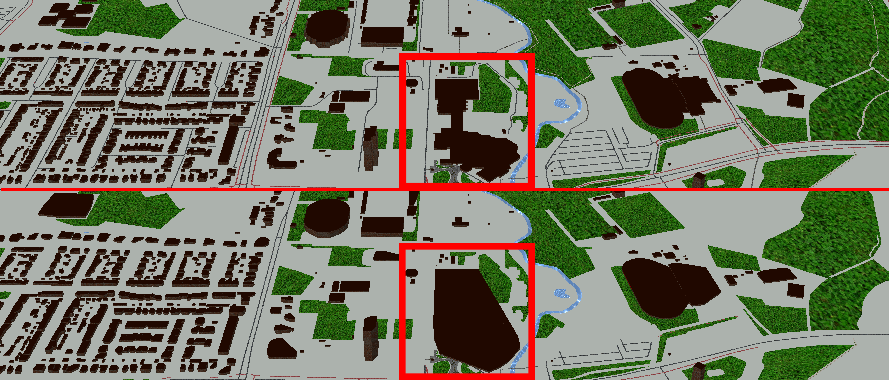
\includegraphics[width=\textwidth]{Simplification}
\caption{Top: detailed version, Bottom: Simplified version}
\label{fig:Simplification}
\end{figure}

\section{GPU usage}
\label{sec:GPUUsage}
We have tested our system with 2 versions of the data set. The first data set is a single node tree with whole Eindhoven in this single node, thus only the highest level of detail is used. So the visualize application can only render the single node. The second version was a set where Eindhoven was divided in the tree, so the visualize application could choose which nodes it can render. Also in the second version, the error per meter was set on 500.

figure 4 shows the GPU (Graphics Processing Unit) load for the 2 tests and also what the GPU load is when the application isn’t running. When running the test with a single node the GPU load is a lot higher than for the multi node test.

figure 5 presents the memory usage on the GPU for the 2 tests and also shows the memory usage when the application isn’t running. The single node dataset uses a bit more memory than the multi node dataset. Also when the application doesn’t run, the system also uses video memory.

\section{Limitations}
\label{sec:Limitations}
The height of buildings is determined with the building surface area of the building. If the building has an underground structure like underground parking garage, then the building is extremely high. The surface area of the geographic polygon is very small against the surface area of the whole building. This limitation expresses itself by generating very high building, while in reality the building above the ground is very low.

The width of a road is also approximated, by using meta-data. Sometimes this metadata isn’t available or wrong, which results in a different width. Also the road could have wider or smaller lanes.

